\documentclass[10pt,landscape,a4paper]{scrartcl}

%import
\usepackage[german]{babel}
\usepackage[utf8]{inputenc}
\usepackage{multicol}
\usepackage[landscape]{geometry}
\usepackage{hyperref}
\usepackage{graphicx}
\usepackage{listings}
\usepackage{color}
\usepackage{fancyhdr}
\usepackage{paralist}
\usepackage{tikz}
\usetikzlibrary{decorations.markings}

%define color
\definecolor{sectioncolor}{RGB}{0, 0, 255}
\definecolor{subsectioncolor}{RGB}{0, 100, 255}
\definecolor{subsubsectioncolor}{RGB}{0, 150, 255}
\definecolor{b}{RGB}{0, 120, 255} %Default highlite color
\definecolor{p}{RGB}{0, 43, 54} %Dark page color
\definecolor{t}{RGB}{131, 148, 150} %Dark text color
\definecolor{darkgreen}{RGB}{0,150,0}
\definecolor{dkgreen}{rgb}{0,0.6,0}
\definecolor{gray}{rgb}{0.5,0.5,0.5}
\definecolor{mauve}{rgb}{0.58,0,0.82}

%define code color
\lstset{frame=none,
	language=SQL,
	aboveskip=0mm,
	belowskip=0mm,
	showstringspaces=false,
	columns=flexible,
	basicstyle={\small\ttfamily},
	numbers=none,
	numberstyle=\tiny\color{gray},
	keywordstyle=\color{blue},
	commentstyle=\color{dkgreen},
	stringstyle=\color{mauve},
	breaklines=true,
	breakatwhitespace=true,
	tabsize=3
}

%define section color and size
\addtokomafont{section}{\color{sectioncolor}\small\rule{5.5cm}{.5pt}\vspace{-4pt}\\}
\addtokomafont{subsection}{\color{subsectioncolor}\small}
\addtokomafont{subsubsection}{\color{subsubsectioncolor}\small}

%define section spacing
\RedeclareSectionCommands[ 
afterindent = false, 
beforeskip = 0pt, 
afterskip = .1pt 
]{section,subsection,subsubsection}

%format
\geometry{top=1.4cm,left=0.4cm,right=0.4cm}

%no section numbers
\setcounter{secnumdepth}{0}

%define header and footer
\pagestyle{fancy}

\fancyhead[RO]{Zindel Marius}
\fancyhead[LO]{CheatSheet Dbs1}
\fancyfoot[RO]{12.01.2020}
\fancyfoot[LO]{Created with \LaTeX}
\renewcommand\headrulewidth{0pt}
\renewcommand\footrulewidth{0pt}
\headsep = -10pt
\footskip = 3pt
\textheight = 549pt

%new commands
\newcommand{\drule}[3][0]{%
	\tikz[baseline]{\path[decoration={markings,
			mark=between positions 0 and 1 step 2*#3
			with {\node[fill, circle, minimum width=#3, inner sep=0pt, anchor=south west] {};}},postaction={decorate}]  (0,#1) -- ++(#2,0);}}

% -----------------------------------------------------------------------



\begin{document}

%------------------Dark Mode----------------	
%\pagecolor{p}
%\color{t}
%------------------Dark Mode----------------


	\begin{multicols*}{5}
		\setlength{\columnseprule}{0.4pt}
		\footnotesize
\section{Begriffe}
\textcolor{b}{DB:} Datenbasis, strukturierte Daten HD\\
\textcolor{b}{DBMS:} Datenbankmanagementsystem\\
\textcolor{b}{DBS:}(Datenbanksystem) DBMS + n* DB\\
\textcolor{b}{Datenkonsistenz:} korrekte Daten\\
\textcolor{b}{Datensicherheit:} vor phy. Verlust\\
\textcolor{b}{Datenschutz:} vor unberecht. Zugriff\\
\textcolor{b}{Funktionen DBMS:} Transaktionen, Mehrbenutzerbetrieb, Sicherheit, Backup \& Recovery, Generische Datenstrukturen\\
\textcolor{b}{Vorteile DBMS:} Skalierbar, Sicherheit, Integrität, Live-Abfragen, Kapslung\\



\section{DB-Modelle}
\subsubsection{Hierarchisches Datenbankmodell}
Die zu speichernden Informationen werden in \textcolor{b}{Hierarchie} organisiert. Auch die beziehungen zwischen den Daten werden als Hierarchie gespeichert.\\
\textcolor{red}{Nachteile:} Es ist sehr schwer die Welt "Hierarchisch" darzustellen. Änderungen sind sehr schwer vorzunehmen. Trennung von Daten ist sehr schwer
\subsubsection{Netzwerkmodell}
Die zu speichernden Informationen werden in vernetzten Hierarchien	organisiert. Beziehungen innerhalb der Hierarchie werden zusammen mit den Daten gespeichert, was eine \textcolor{b}{Mehrfachbeziehung} von Elementen möglich macht.\\
\textcolor{red}{Nachteil:} Effiziente Anwendungen nur möglich in Kenntnis der komplexen Netzwerk-Datenstruktur. Dadurch besteht eine starke Abhängigkeit zwischen Daten und Anwendung.
\subsubsection{Relationenmodell}
Alle Informationen werden als unstrukturierte Daten in Form von \textcolor{b}{Tabellen} gespeichert. Dadurch ist alles \textcolor{b}{sehr flexibel} und all mögliche abfragen lassen sich realisieren. Ebenfalls ist eine \textcolor{b}{klare Trennung} zwischen den Daten und Anwendungen möglich.
\textcolor{red}{Nachteile:} Unterschiede zwischen den Typensystemen der DB und den Anwendungen ist schwer zu konvertierten. 
\subsubsection{Objektrelationales Modell}
Ist eine weiterentwickeln des rel. Datenmodells. Es können aber auch zusätzlich \textcolor{b}{Methoden} gespeichert werden. Tabellen können verschachtelt werden (1. Normalform muss nicht erfüllt sein). Benutzerdefinierte Typen sowie Tabellen-Vererbung können erstellt werden.
\columnbreak

\section{ER-Modell}
Das ER-Modell modelliert den interessierenden Ausschnitt der 'Welt' grafisch als Entitätsmengen (Typen) mit den Beziehungen zwischen diesen Mengen (Assoziationen). Es ist vergleichbar mit dem Domain Model.
	\vspace{-15pt}
\begin{center}
	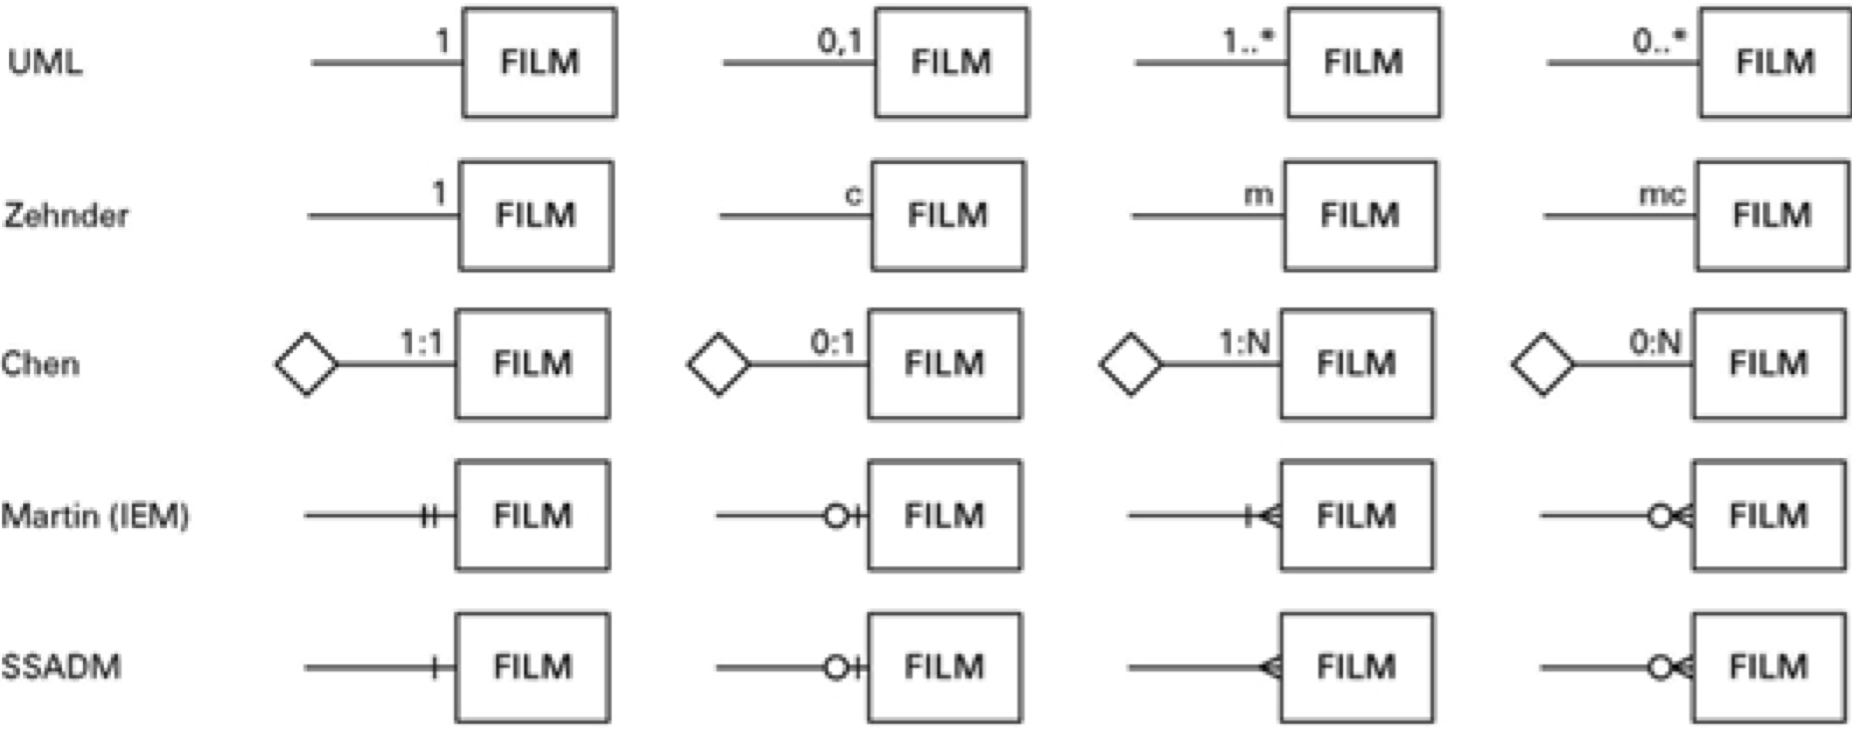
\includegraphics[scale=.17]{Graphic/Vergleich_notationen}
\end{center}
	\vspace{-15pt}
\section{UML}
\textcolor{b}{UML} erweitert die ER-Technik um dynamische Aspekte.
	\vspace{-8pt}
\begin{center}
	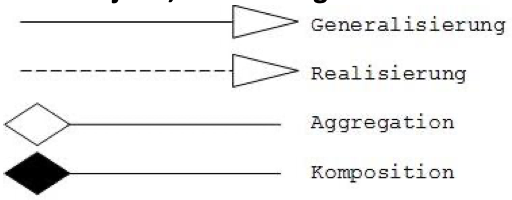
\includegraphics[scale=.4]{Graphic/UML}
\end{center}
	\vspace{-8pt}
\textcolor{b}{Aggregation:} Kann in mehreren vorkommen und wird nicht gelöscht.\\
\textcolor{b}{Komposition:} Wird Vater gelöscht, dann auch Kind. Kann nur 0-1 haben

%\columnbreak
\vspace{-8pt}
\section{Relationale Schreibweise}
	\begin{center}
		\begin{tabular}{|l|}
			\hline
			Student\\
			\hline
			+ Name TEXT\\
			+ Wohnort TEXT\\
			\hline
		\end{tabular}
\vspace{-8pt}
	\end{center}
	\texttt{Student (\underline{StudID} INT, \\
		Name TEXT NOT NULL,\\
		Wohnort TEXT NOT NULL)}
	\vspace{-10pt}
	\drule{5cm}{1pt}
	\vspace{-8pt}
	\begin{center}
		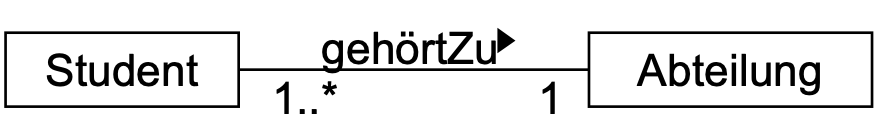
\includegraphics[scale=.25]{Graphic/uml1_n}
	\end{center}
	\vspace{-8pt}
	\texttt{Abteilung (\underline{abtId}, Name)\\
		Student (\underline{StudId} INT, \\
		AbtId NOT NULL REFERENCES Abteilung)}
	\vspace{-6pt}
\drule{5cm}{1pt}
	\begin{center}
		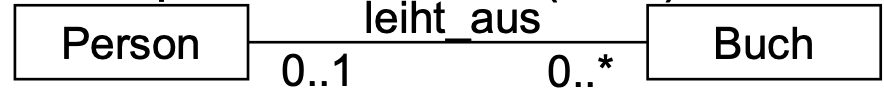
\includegraphics[scale=.25]{Graphic/uml_opt}
	\end{center}
	\vspace{-8pt}
	\texttt{Person (\underline{PId}, Name NOT NULL)\\
		Buch (\underline{BuchId} INT, \\
		Ausleiher NULL REFERENCES Person)}
	\vspace{-8pt}
\drule{5cm}{1pt}
	\begin{center}
		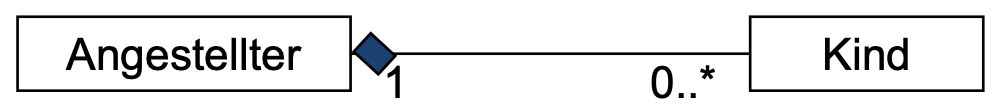
\includegraphics[scale=.25]{Graphic/UML_Aggregation}
	\end{center}
	\vspace{-8pt}
	\texttt{Angestellter (\underline{AngId}, Name NOT NULL)\\
		Kind (\underline{AngId} REFERENCES Angestellter NOT NULL, Name)}
	\vspace{-8pt}
\drule{5.5cm}{1pt}
	\begin{center}
		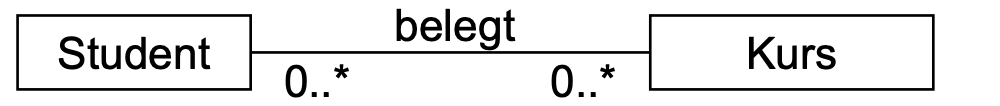
\includegraphics[scale=.25]{Graphic/UML_n_m} \newline\newline\newline
	\end{center}
	\vspace{-30pt}
	\texttt{Student (\underline{StudId} , Name NOT NULL)\\
		Kurs (\underline{KursId},Bezeichnung NOT NULL)\\
		Belegung (\underline{StudId} REFERENCES Student,
		\underline{KursId} REFERENCES Kurs)}
	\vspace{-8pt}
\drule{5cm}{1pt}
	\begin{center}
		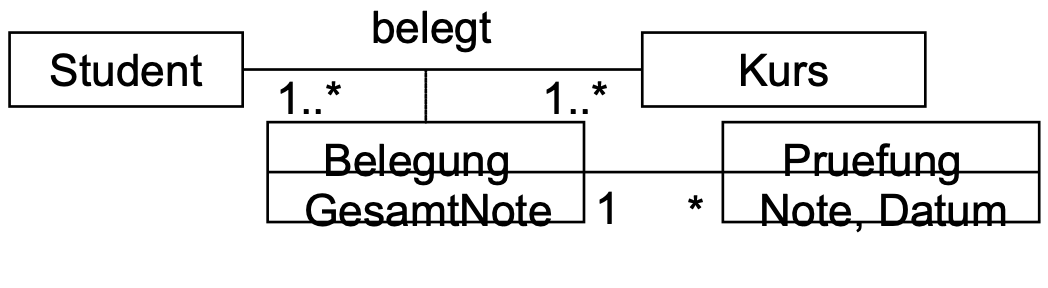
\includegraphics[scale=.2]{Graphic/UML_ass_Klassen}
	\end{center}
	\vspace{-8pt}
	\texttt{Student (\underline{StrudId}, Name)\\
		Kurs (\underline{KursId}, Bez.)\\
		Belegung (\underline{StudId, KursId}, GesamtNote)\\
		Prüfung (\underline{StudId} REFERENCES Belegung, \underline{KursId} REFERENCES Belegung, \underline{Datum}, Note NOT NULL)}
	\vspace{-8pt}
\drule{5.5cm}{1pt}
	\begin{center}
		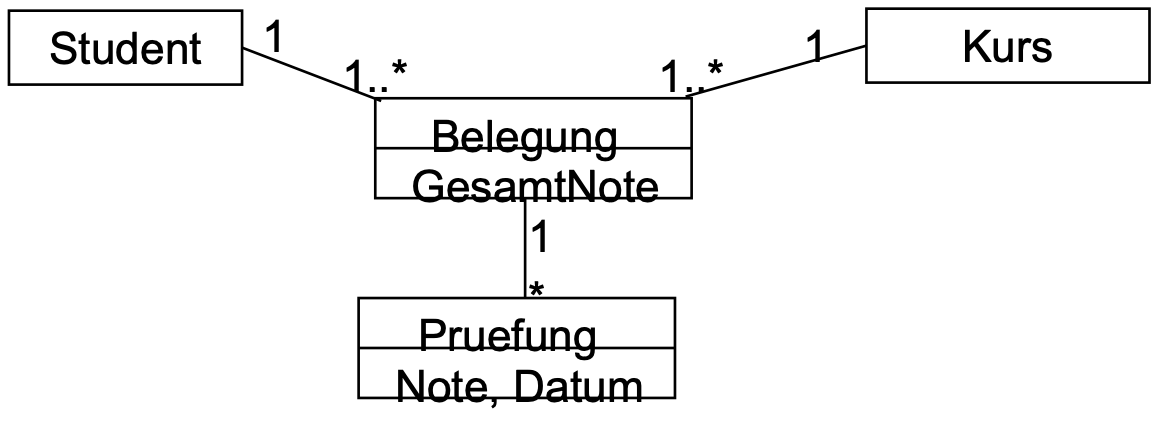
\includegraphics[scale=.2]{Graphic/UML_ass_Klassen_b}
	\end{center}
	\texttt{Student (\underline{StrudId}, Name)\\
		Kurs (\underline{KursId}, Bez.)\\
		Belegung (\underline{BelId}, StudId, KursId, GesamtNote)\\
		Prüfung (\underline{BelId, Datum} Note NOT NULL)}
%\columnbreak

\section{Vererbung}
Die \textcolor{b}{Superklasse} und \textcolor{b}{Subklasse} wird auf eine Tabelle abgebildet,\\
Primärschlüssel der Subklassen-Tabellen \textcolor{b}{=} Primärschlüssel der Superklasse.\\
Der \textcolor{b}{Primärschlüssel} der Subklassen ist zugleich Fremdschlüssel.\\
\textcolor{darkgreen}{Vorteil:} Flexibelste Lösung, Redundanzfrei, geeignet für überlappende Vererbung\\
\textcolor{red}{Nachteil:} Viele Tabellen, Komplexe Zugriffe, Zusätzlicher Typ-Attribut
\texttt{Fahrzeug (\underline{FzgId} INT, Marke STRING, Gewicht DECIMAL,\\
	FzgTyp INT NOT NULL)\\
	PKW (\underline{FzgID} REFERENCES Fahrzeug, AnzPlaetze INT NOT NULL)}\\
\drule{5.5cm}{1pt}
\textcolor{b}{Eine Tabelle pro Klasse}\\
\textcolor{darkgreen}{Vorteil:} Einfache Zugriffe auf die Tabellen\\
\textcolor{red}{Nachteil:} Semantikverlust (nicht mehr klar was gemeinsam ist), Schlüssel-Eindeutigkeit separat kontrollieren, keine Überlappende Vererbung
\drule{5.5cm}{1pt}
Nur eine ''Super''-Tabelle\\
\textcolor{darkgreen}{Vorteil:} Einfache Zugriffe auf die Tabellen\\
\textcolor{red}{Nachteil:} Viele NULL-Werte pro Tupel, 3. oder höhere Normalform verletzt

\section{Normalform}
Die Redundanzfreiheit wird geprüft:\\
\textcolor{b}{1.NF:} Wertebereiche der Attribute \textcolor{b}{atomar} (nur ein). Strukturierte Werte wie Mengen, Gruppen, etc. sind also nicht zugelassen.\\
\textcolor{b}{2.NF:} jedes \textcolor{b}{Nichtschlüsselattribut} von \textcolor{b}{jedem Schlüsselkandidaten} voll \textcolor{b}{funktional abhängig} ist. Ein Attribut B ist funktional abhängig vom Attribut A, falls zu jedem Wert von A genau ein Wert von B existiert: jede ISBN gibt es nur ein Buch.\\
\textcolor{b}{3.NF:} kein Nichtschlüsselattribut von irgendeinem Schlüssel über ''Umwege'' abhängig.\\


\section{Window Function}
\begin{lstlisting}
SELECT row_number() over(),
name, salaer, salaer - 
lead(salaer,1,salaer) OVER 
(ORDER BY salaer) FROM 
angestellter ORDER BY 2 DESC;
\end{lstlisting}

\section{Common Table Expressions}
Wie temp. Tabellen, sind Hilfqueries
\begin{lstlisting}
WITH angestprojekten AS (
SELECT a.persnr, a.name, a.chef, 
a.abtnr, proj.bezeichnung FROM
angestellter a JOIN 
projektzuteilung pz ON a.persnr 
= pz.persnr
SELECT * FROM angestprojekten;
\end{lstlisting}
\section{Recursive Query}
Dazu muss \texttt{WITH RECURSIVE} zusätzlich geschrieben werden.
\begin{lstlisting}
WITH RECURSIVE query_name (column_name) AS (
-- Nicht rekursiver Teil.....
UNION ALL 
-- Recursiver Teil...) 
SELECT c1,c2 FROM query_name;

\end{lstlisting}
\section{View}
\begin{lstlisting}
CREATE VIEW AngPublic (Persnr, 
Name, Tel, Wohnort) AS SELECT 
Persnr, Name, Tel, Wohnort FROM 
Angestellter; -- Create View

SELECT * FROM AngPublic; -- Use
\end{lstlisting}
\columnbreak

\section{Join}
\begin{tabular}{p{1.5cm}|p{3.34cm}}
	\raisebox{-\totalheight}{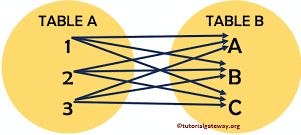
\includegraphics[scale=.15]{Graphic/CrossJoin}}&\textcolor{b}{Cross Join}\newline (Kartesisches Produkt) \begin{lstlisting}
SELECT * FROM ang, 
abt;
	\end{lstlisting}\vspace{-10pt}\\
	\hline
	\raisebox{-\totalheight}{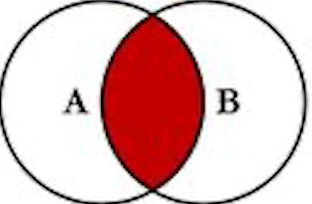
\includegraphics[scale=.3]{Graphic/InnerJoin}}&\textcolor{b}{Inner Join}
	\begin{lstlisting}
SELECT * FROM tab1 
JOIN tab2 ON 
tab1.spalte = 
tab2.spalte;			
	\end{lstlisting}\vspace{-10pt}\\
	\hline
	\raisebox{-\totalheight}{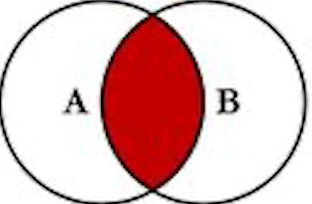
\includegraphics[scale=.3]{Graphic/InnerJoin}}&\textcolor{b}{Natural Join}\newline automatisch Spalten, mit gleichen Namen.
	\begin{lstlisting}
SELECT * FROM 
tabelle1 NATURAL 
JOIN tabelle2;
	\end{lstlisting}\vspace{-10pt}\\
	\hline
	\raisebox{-\totalheight}{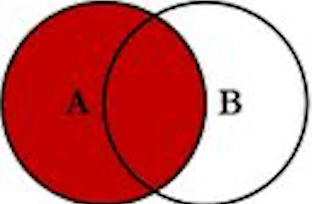
\includegraphics[scale=.3]{Graphic/LeftOuterJoin}}&\textcolor{b}{Left Join}\newline wie Inner, nur + alle Elemente links.
	\begin{lstlisting}
SELECT * FROM 
tabelle1 LEFT 
JOIN tabelle2 ON 
tabelle1.spalte = 
tabelle2.spalte; 
	\end{lstlisting}\vspace{-10pt}\\
	\hline
	\raisebox{-\totalheight}{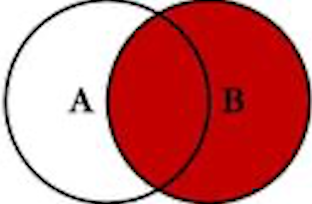
\includegraphics[scale=.3]{Graphic/RightOuterJoin}}&\textcolor{b}{Right Join}\newline wie Inner, nur + alle Elemente rechts.
	\begin{lstlisting}
SELECT * FROM 
tabelle1 RIGHT 
JOIN tabelle2 ON 
tabelle1.spalte = 
tabelle2.spalte;
	\end{lstlisting}\vspace{-10pt}\\
	\hline
	\raisebox{-\totalheight}{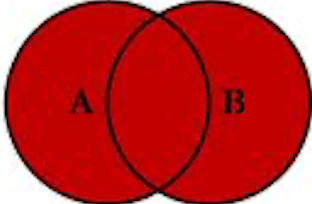
\includegraphics[scale=.3]{Graphic/FullOuterJoin}}&\textcolor{b}{Full Outer Join}\newline Verknüpfung von Left und Right Join. 
	\begin{lstlisting}
SELECT * FROM tab1
FULL JOIN tab2 ON 
tab1.spalte = 
tab2.spalte;
	\end{lstlisting}\vspace{-10pt}\\
	\hline
	\raisebox{-\totalheight}{
\includegraphics[scale=.05]{Graphic/SelfJoin}}&\textcolor{b}{Self Join}\newline Tabelle mit sich selbst. 
	\begin{lstlisting}
SELECT * FROM tab1 
a, tab1 b WHERE 
a.chefid = b.id;
	\end{lstlisting}\vspace{-10pt}\\
\end{tabular}

\section{ANSI 3-Ebenen}
\begin{tabular}{p{1cm}|p{3.8cm}}
\textcolor{b}{Logische Ebene}&Logische Strukur der Daten\\
\hline
\textcolor{b}{Interne Ebene}&Speicherstrukturen\\
\hline
\textcolor{b}{Externe Ebene}&Sicht einer Benutzerklasse auf Teilmenge der Daten\\
\hline
\textcolor{b}{Mapping}&Zw. Ebenen Abbildung nötig\\
\hline
\end{tabular}
\columnbreak

\section{SQL-Abfragen}
Mit \textcolor{b}{\texttt{DISTINCT}} werden entstehende Duplikate ausgeschlossen.\vspace{-8pt}\\
\vspace{-2pt}
\textcolor{darkgreen}{\drule{5.5cm}{1pt}}
Mit \textcolor{b}{\texttt{LIKE}} wird nach einem String-Muster gesucht, wobei \% (0 bis n beliebige Zeichen) oder \_ (genau ein beliebiges Zeichen) eingesetzt werden können.\vspace{-8pt}\\
\vspace{-2pt}
\textcolor{darkgreen}{\drule{5.5cm}{1pt}}
\textcolor{b}{Aggregatfunktionen} liefern als Resultat nur eine Zeile. NULL-Werte werden übersprungen.
\begin{lstlisting}
SELECT AVG( salaer ) FROM ang; 
\end{lstlisting}\vspace{-8pt}
\textcolor{darkgreen}{\drule{5.5cm}{1pt}}
\textcolor{b}{HAVING-Klausel} kann nur nach einer GROUP-BY-Klausel stehen.
\begin{lstlisting}
GROUP BY abtnr HAVING AVG(salaer)
 >= 7000 ORDER BY AVG(salaer);
\end{lstlisting}\vspace{-8pt}
\textcolor{darkgreen}{\drule{5.5cm}{1pt}}
\textcolor{b}{IN} Liste der Angestellten (Name), die in keinem Projekt mitarbeiten:
\begin{lstlisting}
SELECT name FROM ang WHERE 
persnr NOT IN (SELECT DISTINCT ..
\end{lstlisting}\vspace{-8pt}
\textcolor{darkgreen}{\drule{5.5cm}{1pt}}
\textcolor{b}{EXISTS} Liste der Angestellten, die in mindestens einem Projekt mitarbeiten:
\begin{lstlisting}
SELECT name FROM ang a WHERE
EXISTS ( SELECT * FROM projzut
WHERE persnr = a.persnr); 
\end{lstlisting}\vspace{-8pt}
\textcolor{darkgreen}{\drule{5.5cm}{1pt}}
\textcolor{b}{ANY} Gesucht sind die 'Marketing'-Angestellten, die weniger als irgend einer der Entwickler verdienen: ANY liefert für jedes solche Tupel 'true'.						
\begin{lstlisting}
SELECT ang.name, ang.salaer FROM 
angestellter ang INNER JOIN 
Abteilung Abt ON ang.abtnr = 
abt.abtnr WHERE abt.name = 
'Marketing' AND ang.salaer < ANY 
( SELECT salaer FROM angestellter 
ang1 INNER JOIN Abteilung abt1
ON ang1.abtnr = abt1.abtnr
WHERE abt1.name='Entwicklung');			
\end{lstlisting}\vspace{-18pt}
\textcolor{darkgreen}{\drule{5.5cm}{1pt}}
\textcolor{b}{ALL} Gesucht sind die 'Marketing'-Angestellten, die mehr als jeder der Entwickler verdienen:
ALL liefert für jedes solche Tupel 'true'
\begin{lstlisting}
SELECT ang.salaer, ang.salaer 
FROM angestellter ang INNER JOIN 
abteilung abt ON ang.abtnr = 
abt.abtnr WHERE abt.name = 
'Marketing' AND ang.salaer > ALL
(SELECT salaer FROM angestellter 
ang1 INNER JOIN Abteilung abt1 
ON ang1.abtnr=abt1.abtnr 
WHERE abt1.name='Entwicklung');
\end{lstlisting}\vspace{-8pt}
\textcolor{darkgreen}{\drule{5.5cm}{1pt}}
\textcolor{b}{count (*)$>$0} $\rightarrow$ True oder False

\columnbreak
\section{Security}

\begin{compactitem} [$\bullet$]
	\item Identifizierung und Authentisierung von Benutzern 
	\item Überprüfung der Benutzerprivilegien für Ausführung von Systemoperationen.
	\item Kontrolle der Benutzung von CPU, Disk.
\end{compactitem}
\textcolor{b}{Benutzern} sind Privilegien zugeordnet für Datenbankoperationen.
	\begin{compactitem}[$\bullet$]
	\item \textcolor{b}{Rollen} gelten über alle \textcolor{b}{alle Datenbanken}
	\item \textcolor{b}{Schemas} fassen \textcolor{b}{Datenbank-Objekte} \textcolor{b}{zusammen} in einer \textcolor{b}{bestimmten Datenbank}
	\item Eine \textcolor{b}{Datenbank} kann \textcolor{b}{n * Schemas} haben 
	\item Eine \textcolor{b}{Rolle} kann \textcolor{b}{n * Schemas} besitzen
	\item \textcolor{b}{Ohne Angabe} eines \textcolor{b}{Schema-Namens} werden \textcolor{b}{alle Objekte im Default Schema} ''public'' erzeugt
\end{compactitem}
\begin{lstlisting}
CREATE ROLE angproj WITH LOGIN 
PASSWORD 'angproj';
GRANT INSERT ON TABLE 
"Angestellter" TO "angproj"; 
\end{lstlisting}
\vspace{-10pt}
\drule{5.5cm}{1pt}
Systemprivilegien legen fest, welche Operationen ein Benutzer ausführen darf.
\begin{compactitem} [$\bullet$]
	\item \textcolor{b}{\texttt{REATEDB}}: Erlaubt dem Benutzer Datenbanken auf Server zu erstellen.
	\item \textcolor{b}{\texttt{CREATEROLE}}: Erlaubt der Rolle / Benutzer neue Rollen/Benutzer zu erstellen.
	\item \textcolor{b}{\texttt{NOREADDB}} und \textcolor{b}{\texttt{NOCREATEROLE}} sind Negationen davon.
\end{compactitem}
\vspace{-10pt}
\drule{5.5cm}{1pt}
Mit \textcolor{b}{\texttt{REVOKE}} kann der Benutzer,  das Recht wieder entziehen.
\begin{lstlisting}
REVOKE [GRANT OPTION FOR]{
privilege [, privilege...]|ALL 
[PRIVILEGES]} ON object FROM
{user[, user...]|GROUP 
group|PUBLIC} [CASCADE|RESTRICT];
\end{lstlisting}
\vspace{-10pt}
\drule{5.5cm}{1pt}
\textcolor{b}{Gruppen} sind \textcolor{b}{Sammlungen} von logisch \textcolor{b}{zusammengehörenden Benutzern}. Gruppen können \textcolor{b}{Objektprivilegien zugeordnet} werden. \textcolor{b}{Benutzer} können \textcolor{b}{Gruppen zugeordnet} werden, die Benutzer erhalten dann die \textcolor{b}{in den Gruppen definierten Privilegien}.
\begin{lstlisting}
CREATE ROLE angmanager;
GRANT SELECT, UPDATE
ON angproj.angestellter TO 
angmanager;
GRANT angmanager TO Blake; 
\end{lstlisting}
\columnbreak
\section{Transaction}
\begin{tabular}{p{.1cm} | p{1.1cm} | p{3.2cm} }
	A&Atomicity&entweder vollständig oder gar nicht\\
	\hline
	C&Consis-tency&führt Daten von konsistenten Zustand in einen anderen\\
	\hline
	I&Isolation&Soll ausgeführt werden, als sei sie isoliert\\
	\hline
	D&Durability&Änderungen einer Transaktion gehen nicht durch Fehler verloren\\
\end{tabular}
\drule{5.5cm}{1pt}
	Mit \textcolor{b}{\texttt{ROLLBACK}} oder \textcolor{b}{\texttt{ABORT}} kann Transaktion abgebrochen werden. Mit \textcolor{b}{\texttt{SAVEPOINT SavepointName}} kann aktuelle Punkt gespeichert werden. Mit \textcolor{b}{\texttt{ROLLBACK TO SavepointName}} kann zurückgesprungen werden. Nach \textcolor{b}{\texttt{COMMIT}} oder \textcolor{b}{\texttt{ROLLBACK}} gibt DBMS sämtliche Ressourcen frei.
\subsection{Serialisierbarkeit}

\begin{center}
	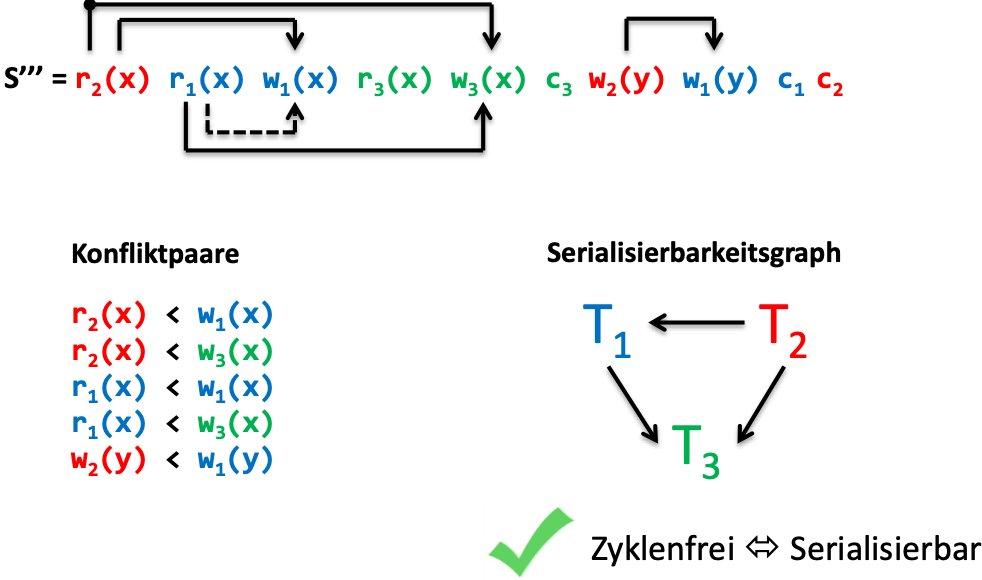
\includegraphics[scale=.3]{Graphic/serialisierbarkeitsgraf2}
\end{center}
\vspace{-10pt}
\subsection{Locking Protokolle}
\begin{compactitem} [$\bullet$]
	\item \textcolor{b}{Exclusive Lock (xlock)}\\
	Schreib- und Lesezugriffe sind gesperrt
	\item \textcolor{b}{Shared Lock (slock)}\\
	Nur Lesezugriffe sind gesperrt (mehrere können S-Lock auf Objekt halten)
\end{compactitem}
\subsection{Iso-Level}
\begin{compactitem} [$\bullet$]
	\item \textcolor{b}{READ UNCOMMITTED} (\textcolor{red}{schwächste})\\
	Lesezugriffe nicht synchronisiert (keine Read-Locks) 
	\item \textcolor{b}{READ COMMIETT}\\
	Lesezugriffe nur kurz /temporär synchronisiert
	\item \textcolor{b}{REPEATABLE READ}\\
	Einzeln zugegriffene Rows sind synchronisiert
	\item \textcolor{b}{SERIALIZABLE} (\textcolor{darkgreen}{stärkste})
	Vollständige Isolation
\end{compactitem}
\begin{tabular}{|p{1.9cm}|p{.7cm}|p{.7cm}|p{.7cm}|}
	\hline
	Isolation \newline Level&Dirty Read&Fuzzy Read&Phan-tom\\
	\hline
	\hline
	READ UNCOMMITED&\textcolor{red}{mögl.}&\textcolor{red}{mögl.}&\textcolor{red}{mögl.}\\
	\hline
	READ \newline COMMITTED&\textcolor{darkgreen}{nicht mögl.}&\textcolor{red}{mögl.}&\textcolor{red}{mögl.}\\
	\hline
	REPEATABLE READ&\textcolor{darkgreen}{nicht mögl.}&\textcolor{darkgreen}{nicht mögl.}&\textcolor{red}{mögl.}\\
	\hline
	SERIALI-ZABLE&\textcolor{darkgreen}{nicht mögl.}&\textcolor{darkgreen}{nicht mögl.}&\textcolor{darkgreen}{nicht mögl.}\\
	\hline
\end{tabular}
\textcolor{b}{Dirty Read} Lese Daten von anderer nicht committed Transaktion.\\
\textcolor{b}{Fuzzy Read} Gelesene Daten ändern sich plötzlich durch andere nebenläufige Transaktionen\\
\textcolor{b}{Phantom Read} INSERT oder DELETE von nebenläufigen Transaktionen. Tritt in Postgres nicht\\ auf $\rightarrow$ Snapshot Isolation!
\vspace{-8pt}
\section{Recovery}
Änderungen der Transaktionen in Logfiles geschrieben.
\begin{compactitem}[$\bullet$]
	\item Implementation des globalen Undo's und des globalen Redo's nach einem Fehlerfall.
	\item Checkpoint: DBMS schreibt alle modifzierten Pages auf Disk und macht Checkpoint Eintrag ins Log
	\item globales REDO: Die Wirkung sämtliche Transaktionen, welche mit einem Commit abgeschlossen
	wurden, darf nicht verlorengehen gehen
	\item globales UNDO: Die Wirkung sämtliche Transaktionen, welche noch nicht mit einem Commit
	abgeschlossen wurden, müssen rückgängig gemacht werden. 
\end{compactitem}
\vspace{-8pt}
\drule{5.5cm}{1pt}
\begin{compactitem} [$\bullet$]
	\item \textcolor{b}{Logischer Backup} (mit pg\_dump)\\
	Blockiert keine schreibende und lessende Transaktionen
	\item \textcolor{b}{Physikalisches Backup}\\
	Datenbank muss heruntergefahren warden – ist aber schneller
	\item \textcolor{b}{Cloud Backup}\\
	Alle Cloud Provider bieten Backups an in ihren PostgreSQL-Angeboten
\end{compactitem}
\vspace{-8pt}
\section{Indexe}
Arten von Indexen:
\begin{compactitem} [$\bullet$]
	\item ISAM
	\item B-Bäume
	\item B+ -Bäume
	\item Hash
\end{compactitem}
\textcolor{b}{Primär-Index:} Index mit Primärschlüssel\\
\textcolor{b}{Sekundär-Indexe:} Alle anderen Indexe\\
\textcolor{b}{Zusammengesetzter Index} über mehrere zusammengesetzte Attribute/Kolonnen:
\begin{lstlisting}
CREATE INDEX angestellter_name 
_idx ON angestellter (vorname, 
nachname); 
\end{lstlisting}
\drule{5.5cm}{1pt}					
\textcolor{b}{B-tree Index mit zusätzlicher INCLUDE-Klausel} als «Zusatzfracht». INCLUDE gibt Liste von Attriuten an, die als Nicht-Schlüsselteil in den Index aufgenommen werden.
\begin{lstlisting}
CREATE INDEX magic_idx
ON test (nr,id) INCLUDE (txt); 
\end{lstlisting}
\drule{5.5cm}{1pt}	
\textcolor{b}{Partieller Index} mit WHERE-Klausel.
\begin{lstlisting}
CREATE INDEX mytable_col_part_idx
ON mytable (col)
WHERE archived IS NOT NULL; 
\end{lstlisting}
\drule{5.5cm}{1pt}
\textcolor{b}{Funktionaler Index} mit Funktion
\begin{lstlisting}
CREATE INDEX angestellter_lower_ 
name_idx ON angestellter 
(lower(name)); 
\end{lstlisting}
\drule{5.5cm}{1pt}
\textcolor{b}{B-Baum} Eigenschaften: Geeignet für Hintergrundspeicher, viele Index-Bedürfnisse und Fast optimal für verschiedene Queries und Einfügen.\\
Ein \textcolor{b}{B+-Baum} ist ein B-Baum, bei dem nur die Blätter Daten enthalten und zudem verkettet sind (z.B. als Linked List). Die Verkettung erlaubt schnelle Iterationen.\\
\textcolor{b}{Logische Optimierung:} Abfrage so umformulieren, dass sie dasselbe Resultat liefert aber effizienter berechnet werden kann.
\begin{compactitem} [$\bullet$]
	\item WHERE“-Statements so früh wie möglich, um Zwischenergebnisse klein zu halten
	\item Basisoperationen sollten ohne Zwischenspeicherung von Zwischenrelationen realisiert werden
	\item Nur Berechnungen ausführen, die auch einen Beitrag zum Gesamtergebnis liefern
	\item Zusammenfassen gleicher Teilausdrücke
\end{compactitem}
\textcolor{b}{Der Planer}
\begin{compactitem} [$\bullet$]
	\item \textcolor{b}{Full Table Scan}\\
	Bsp: \texttt{SELECT * FROM angestellter;}
	\item \textcolor{b}{Index Scan}\\
	Falls in der WHERE-Klausel ein Attribut ist, zu dem es einen Index gibt. Bsp: \texttt{SELECT * FROM angestellter WHERE abtnr = 2}
	\item \textcolor{b}{Bitmap Index Scan}\\
	Ein Bitmap Index Scan lädt alle Tupel-Zeiger auf einmal aus dem Index, benutzt eine Bitmap-Struktur, um sie im Hauptspeicher zu sortieren und lädt die Tabellen-Tupel entsprechend der physischen Speicherreihenfolge.
	\item \textcolor{b}{Index Only Scan}
	Falls ein Attribut in der Projektion vorkommt. Bsp: \texttt{SELECT abtnr FROM angestellter WHERE abtnr=2;}
	\item \textcolor{b}{Nested loop join}\\
	Die rechte tabelle wird für jede Zeile der linken Tabelle gescannt. Ist einfach, kann aber zeitaufwändig sein.
\end{compactitem}
	\end{multicols*}
\end{document}}
